To consider possibilities and limitations of the our approach later we introduce an example machine learning streaming problem.

Let's suppose that we have an application that consists of the frontend and backend sides.
They both log user's queries and send logs to the log service.
For simplicity, let's assume that every user query produces one log entity from the frontend and one log entity from the backend, and they have equal and unique query id.

The log entities have the following structure (ts stands for the timestamp):

\begin{tabular}{|l|llll|}
    \hline
    \textbf{frontend} & version & queryId & userId & ts \\
    \hline
\end{tabular}

\vspace{0.1em}

\begin{tabular}{|l|lllll|}
    \hline
    \textbf{backend} & id & queryId & userId & ts & payload \\
    \hline
\end{tabular}

We want to calculate statistics about the time that logged users with new frontend client versions wait for the application answer per user session.
To evaluate when the session ends we will use machine learning model that requires frontend features and users features.

One of the possible solutions is represented on the image TODO. % TODO image ref
Obviously, this solution is not optimal.
Filters are applied to streams too late and number of partitions potentially can be reduced.
To be able to fix it safely we need to know about the requirements and impact of the each operation.

\begin{itemize}
    \item \textbf{joinByQueryId}: Requires queryId field in the elements of both streams.
    \item \textbf{addUsersFeatures}: Requires partition by userId. Users should not be filtered before to get valid statistics. Adds userFeatures field to elements.
    \item \textbf{addFrontFeatures}: Requires only new front versions, adds frontFeatures field to elements in the stream.
    \item \textbf{filterNewFronts}: Leaves only elements with new front versions.
    \item \textbf{modelInference}: Requires front and users features. Sets trigger that signals when to emit data from aggregation.
    \item \textbf{filterAuthorizedUsers}: Requires users features. Filters users that are authorized.
    \item \textbf{stats}: Requires authorized users from new front versions. Also needs session trigger to be set. Sends accumulated statistics to the dashboard.
\end{itemize}

% TODO SQL proof
We see here complex pipeline with stateful operations and streaming triggers management.
It is not possible to describe itin SQL because of it.
Moreover, we see non-trivial operation requirements here, so concrete execution graph specifying will not provide space for optimizations.

% TODO too much lets
Let's consider another pipeline that satisfies requirements: TODO. % TODO image ref
We can see that filters here are maximally close to data sources.
And after permutation of stateful operations we have one less data partition that is rather expensive operation.

In section TODO % TODO number of section
we specify this task using contract-based approach and see, how it helps in optimizations.

% TODO insert properly
% TODO ops naming
\begin{figure}
    \label{fig:running-example-suboptimal}
    \label{fig:running-example-optimal}
    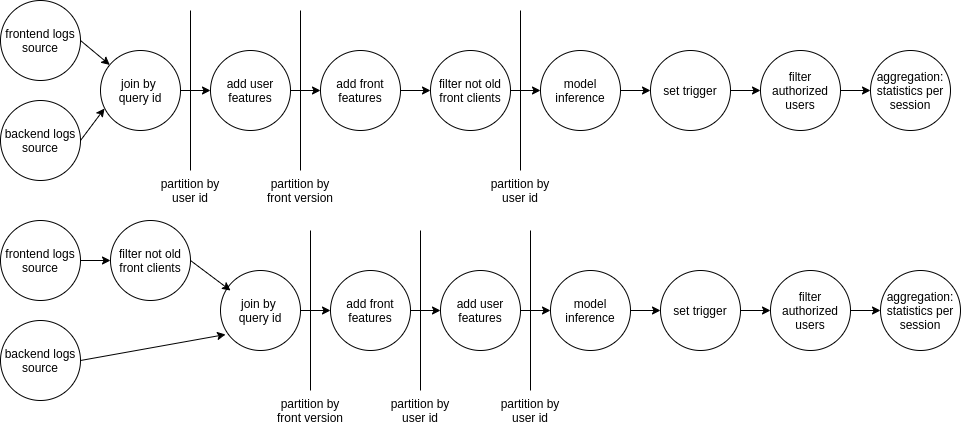
\includegraphics[width=\linewidth]{images/debs-calco-example}
\end{figure}
